% !TeX encoding = UTF-8
% !TeX spellcheck = es_ES
% !TeX root = DB-Conectors.tex

\documentclass[spanish]{DccDiyTools/DccDiyTools}
\usepackage[spanish]{babel}
\usepackage[
type={CC},
modifier={by-sa},
version={4.0},
]{doclicense}

\usepackage[]{DccDiyTools/DccDiyToolsPics}
\usepackage[]{DccDiyTools/DccDiyToolsComponentTables}
\tikzset{
    pics/SmallBoard/.style={
      code = {
        % \draw [step=0.1,very thin, yellow] (-2,-1) grid (2,1);
        % \draw [step=0.5,very thin, red] (-2,-1) grid (2,1);
        % \draw [very thin, green] (-2,-1) grid (2,1);
        \node[inner sep=0pt] at (0,0)
        {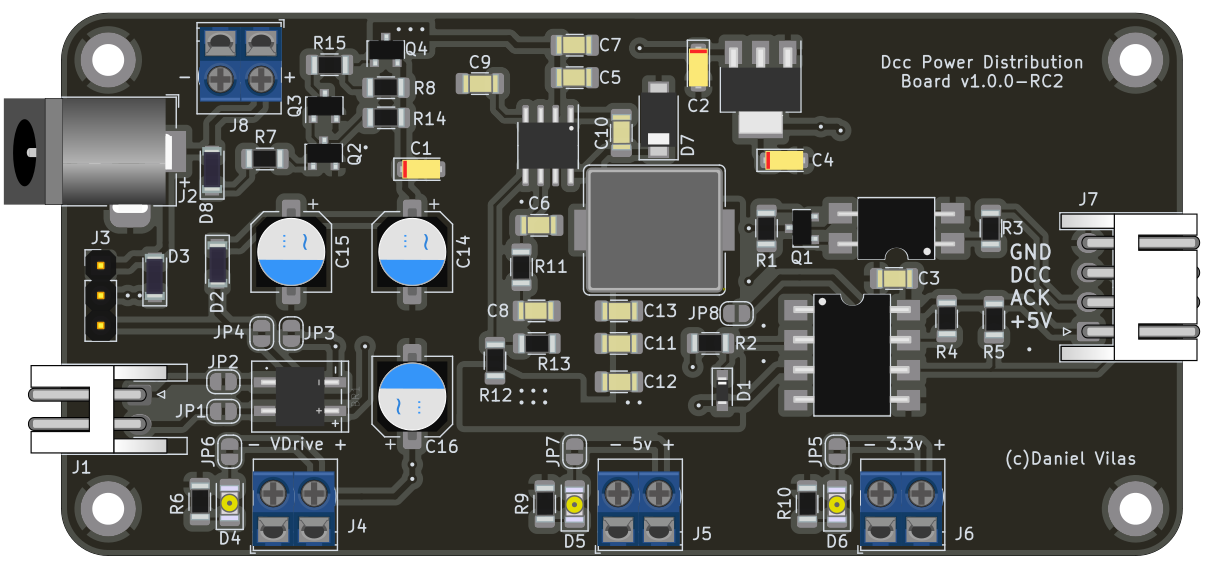
\includegraphics[scale=0.25]{images/front.png}};  


        \node[](-jack) at (-1.35,0.278) {};
        \node[](-terminal) at (-.8,0.65) {};
    }}
}

\tikzset{
    pics/WallAc/.style={
      code = {
    \begin{scope}[shift={(0.25,0)}]
        % \draw [step=0.1,very thin, yellow] (-2,-2) grid (2,2);
        % \draw [step=0.5,very thin, red] (-2,-2) grid (2,2);
        % \draw [very thin, green] (-2,-2) grid (2,2);
        % Mains lead
        \draw[line width=2pt,cap=round, lightgray] (0.05,-0.21) -- (0.05,-0.45);
        \draw[line width=2pt,cap=round, lightgray] (0.275,-0.21) -- (0.275,-0.45);
        % Relief and out cable
        \draw[line width=2pt,cap=round] (-0.5,0.25) -- (-1,0.25);
        \draw[line width=2pt,cap=round,black!75] (-0.55,0.35)--(-0.55,0.15);
        \draw[line width=2pt,cap=round,black!75] (-0.63,0.325)--(-0.63,0.175);
        \draw[line width=2pt,cap=round,black!75] (-0.71,0.3)--(-0.71,0.2);
        \draw[line width=2pt,cap=round,black!75] (-0.79,0.275)--(-0.79,0.225);
        \draw[line width=2pt,cap=round,black!75] (-0.87,0.275)--(-0.87,0.225);

        \draw[line width=2pt,rounded corners=1pt,fill=black!75] (-0.5,0) rectangle +(1,0.5);
        \draw[line width=2pt,rounded corners=1pt,fill=black!65] (-0.1,0) rectangle +(0.5,-0.2);
        % \draw[line width=2pt,cap=round, gray] (0.05,-0.21) -- (0.05,-0.45);
        % \draw[line width=2pt,cap=round,gray] (0.275,-0.21) -- (0.275,-0.45);

        \node[white,scale=0.5] at (0,0.25) {DC Wall};
        \node[](-jack) at (-1.1,0.25) {};
        \node[](-mains) at (.1625,-0.55) {};
    \end{scope}
    }}
}

\title{DB - Conectores}
\subtitle{Conectores usados por DanielBahn}
\author{Daniel Vilas}
\date{Julio 2022}

\dbHeaderTitle{DB - Conectores}
\dbType{M}
\dbDate{22}
\dbCode{001}
\dbStatus{Draft}
\dbVersion{0.1}
%\tikzset{
    pics/SmallBoard/.style={
      code = {
        % \draw [step=0.1,very thin, yellow] (-2,-1) grid (2,1);
        % \draw [step=0.5,very thin, red] (-2,-1) grid (2,1);
        % \draw [very thin, green] (-2,-1) grid (2,1);
        \node[inner sep=0pt] at (0,0)
        {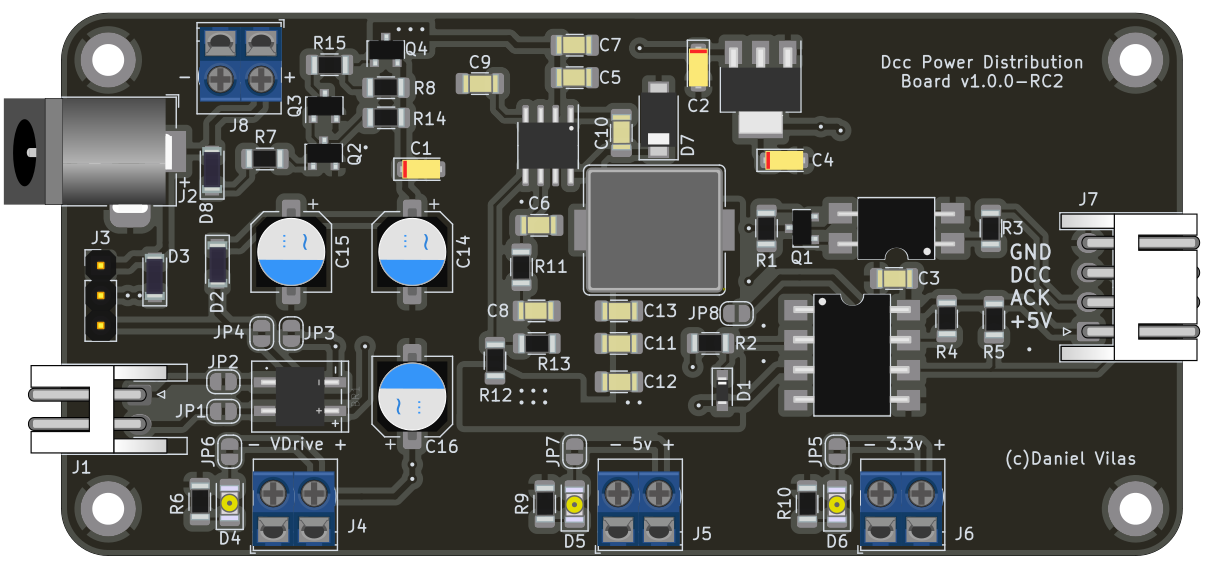
\includegraphics[scale=0.25]{images/front.png}};  


        \node[](-jack) at (-1.35,0.278) {};
        \node[](-terminal) at (-.8,0.65) {};
    }}
}

\tikzset{
    pics/WallAc/.style={
      code = {
    \begin{scope}[shift={(0.25,0)}]
        % \draw [step=0.1,very thin, yellow] (-2,-2) grid (2,2);
        % \draw [step=0.5,very thin, red] (-2,-2) grid (2,2);
        % \draw [very thin, green] (-2,-2) grid (2,2);
        % Mains lead
        \draw[line width=2pt,cap=round, lightgray] (0.05,-0.21) -- (0.05,-0.45);
        \draw[line width=2pt,cap=round, lightgray] (0.275,-0.21) -- (0.275,-0.45);
        % Relief and out cable
        \draw[line width=2pt,cap=round] (-0.5,0.25) -- (-1,0.25);
        \draw[line width=2pt,cap=round,black!75] (-0.55,0.35)--(-0.55,0.15);
        \draw[line width=2pt,cap=round,black!75] (-0.63,0.325)--(-0.63,0.175);
        \draw[line width=2pt,cap=round,black!75] (-0.71,0.3)--(-0.71,0.2);
        \draw[line width=2pt,cap=round,black!75] (-0.79,0.275)--(-0.79,0.225);
        \draw[line width=2pt,cap=round,black!75] (-0.87,0.275)--(-0.87,0.225);

        \draw[line width=2pt,rounded corners=1pt,fill=black!75] (-0.5,0) rectangle +(1,0.5);
        \draw[line width=2pt,rounded corners=1pt,fill=black!65] (-0.1,0) rectangle +(0.5,-0.2);
        % \draw[line width=2pt,cap=round, gray] (0.05,-0.21) -- (0.05,-0.45);
        % \draw[line width=2pt,cap=round,gray] (0.275,-0.21) -- (0.275,-0.45);

        \node[white,scale=0.5] at (0,0.25) {DC Wall};
        \node[](-jack) at (-1.1,0.25) {};
        \node[](-mains) at (.1625,-0.55) {};
    \end{scope}
    }}
}

\begin{document}
\maketitle
\newpage
\section{Introduccion}
% !TeX encoding = UTF-8
% !TeX spellcheck = es_ES
% !TeX root = DB-Conectors.tex
%!TEX root=DB-Conectors.tex
Daniel Bahn es una empresa ficticia para una maqueta de trenes personal. Esta empresa simula ser la gestora de la red ferroviaria dispuesta en dicha maqueta.
Es por tanto el hilo conductor que nos permite entender dicha maqueta.

Para esta maqueta se ha decidido definir una serie de reglas u normativas para facilitar la evolucion de la maqueta propiamente dicha y una metodologia
reutilizable para futuras maquetas.

Este documento es la normativa que deben seguirlas diferentes conexiones electricas entre los elementos principales

La maqueta ha sido diseñada mediante modulos y segmentos que pueden ser conectados y desconectados a voluntad.
Por lo que es importante tener una serie de conectores estandarizados y seguros que faciliten su utilidad

\subsection{Arquitectura}
La maqueta DanielBahn esta dividida en varios segmentos, una version sencilla y reducida
\sidenote{Para entender lo que se quiere explicar aqui} de la misma es:

\begin{figure}[H]
    \centering
    % !TeX encoding = UTF-8
% !TeX spellcheck = es_ES
% !TeX root = ../Esquema.tex
% !TEX root = ../Esquema.tex

\newcommand{\paintBoard}[1][Melon!15]{

    %Base Board
    \draw [fill=#1] (-6,0) rectangle +(3,3)
        (-3,1.5) rectangle +(2,1.5)
        (-1,1.5) rectangle +(2,1.5)
			(1,1.5) rectangle +(2,1.5)
        (6,0) rectangle +(-3,3);
    \draw [fill=Melon!15] (-6,0) rectangle +(3,-3)
        (-3,-1.5) rectangle +(2,-1.5)
        (-1,-1.5) rectangle +(2,-1.5)
        (1,-1.5) rectangle +(2,-1.5)
        (6,0) rectangle +(-3,-3);

}


\newcommand{\paintMain}[2][black]{
    \draw[color=#1,line width=#2] (3,2.1) arc (90:-90:2.1)
    -- (-3,-2.1) arc(-90:-270:2.1) --(3,2.1);
}

\newcommand{\paintStation}[2][black]{
    \draw[color=#1,line width=#2] (5.1,0) --(5.1,-0.3)
        arc(0:-90:2.1) -- (-3,-2.4)
        arc (-90:-180:2.1) -- (-5.1,0);
}

\newcommand{\paintTerminus}[2][black]{
    \draw[color=#1,line width=#2] (-1,-1.8) -- (3,-1.8) arc(-90:90:1.8)
    -- (2.5,1.8) -- (1.2,2.1);

\draw[color=#1,line width=#2] (1.2,-1.8) -- (2.8,-2.1);

}


\newcommand{\paintYard}[2][black]{
	\draw [color=#1,line width=#2] (-2.8,2.1) -- (-1.5,2.4)
		-- (-0.2,2.7);
	\draw [color=#1,line width=#2](-1.5,2.4)
		-- (5,2.4);
	\draw [color=#1,line width=#2](-4,2.7)
		-- (5,2.7);
}

    \caption{Maqueta Simple}
    \label{fig:MaquetaSimple}
\end{figure}

Esta version de la maqueta tiene como objetivo probar diferentes tecnicas
y es por lo tanto muy sencilla en cuanto a diseño de circuito ferroviario.

Estos segmentos necesitan un bus DCC para manejar los trenes, un Bus de corriente
continua para alimentar accesorios y un bus LCB\sidenote{Layout Control Bus} para 
manejar los trenes y recibir informacion de los accesorios.

\begin{figure}[H]
    \centering
    

\begin{tikzpicture}

    %\draw [very thin, green]  (-6,-3) grid (6,3);
    \begin{scope}[shift={(-4.5,0)}] 
        \draw [fill=Melon!15] (-2,-1) rectangle +(4,2);
        \pic[]() at (0,0.25) {RailStraigh=black};
        \node[]() at (0,-0.5){Segmento 1};
    \end{scope}

    \begin{scope}[shift={(0,0)}] 
        \draw [fill=Melon!15] (-2,-1) rectangle +(4,2);
        \pic[]() at (0,0.25) {RailStraigh=black};
        \node[]() at (0,-0.5){Segmento 2};
    \end{scope}

    \begin{scope}[shift={(4.5,0)}] 
        \draw [fill=Melon!15] (-2,-1) rectangle +(4,2);
        \pic[]() at (0,0.25) {RailStraigh=black};
        \node[]() at (0,-0.5){Segmento 3};
    \end{scope}

\end{tikzpicture}
    \caption{Segmentos y Buses}
    \label{fig:ModulosBuses}
\end{figure}

\subsection{Sentidos de circulacion/polarizacion}

El ultimo apartado es definir el sentido de circulacion de la maqueta.
La razon de esto es que Analogico se va hacia delante si por el carril derecho
el voltaje es positivo, por lo que el sentido de circulacion marca la polaridad
de los cables. En digital, es necesario respetar la polaridad de las fases (cables)
por lo que en este caso más que de circulacion, seria de polarizacion.

Por norma general se considera adelante ir en el mismo sentido de lectura, o que es
lo mismo de izquierda a derecha, desde el punto de vista del usuario. Pero esto solo
solo se puede aplicar a maquetas de una sola via (principal) en las que se puede
recorrer la maqueta siguiendo la via.

Para esta maqueta usaremos un Norte Virtual, en el centro de la maqueta. El Sur, sera
el exterior de la maqueta, donde nos situaremos como espectadores, mirando al Norte (centro)
De esta forma, ir de izquerda a derecha, es ir al Este, estemos donde estemos.
Esta direciccion de Oeste a Este se conoce como Eastbound en ingles.

\begin{figure}[H]
    \centering
    \begin{tikzpicture}

    %\draw [very thin, green]  (-6,-3) grid (6,3);
    
    %Base Board
    \draw [fill=Melon!15] (-5,0) rectangle +(3,3)
        (-2,1.5) rectangle +(2,1.5)
        (0,1.5) rectangle +(2,1.5)
        (5,0) rectangle +(-3,3);
    \draw [fill=Melon!15] (-5,0) rectangle +(3,-3)
        (-2,-1.5) rectangle +(2,-1.5)
        (0,-1.5) rectangle +(2,-1.5)
        (5,0) rectangle +(-3,-3);

    %refs 
    % \draw[yellow,line width=2pt] (0,1.8)--(2,1.8); %R1
    % \draw[line width=2pt] (0,2.1)--(2,2.1); %R2
    % \draw[yellow,line width=2pt] (0,2.4)--(2,2.4); %R3
    % \draw[yellow,line width=2pt] (0,2.7)--(2,2.7); %R4
    
    %R2 Circuit
    \draw[line width=2pt] (2,2.1) arc (90:-90:2.1)
    -- (-2,-2.1) arc(-90:-270:2.1) --(2,2.1);

    %R3 Circuit
    \draw[line width=2pt] (4.1,0) --(4.1,-0.3)
        arc(0:-90:2.1) -- (-2,-2.4)
        arc (-90:-180:2.1) -- (-4.1,0);
    
    %R1 Circuit
    \draw[line width=2pt](0,-1.8) -- (2,-1.8) arc(-90:90:1.8)
    -- (1.5,1.8) -- (0.2,2.1);


    \draw[blue] (-1.5,0)--(1.5,0);
    \node[fill=white]at(0,0){Norte};

    \draw[red] (-4.5,-4.5)--(4.5,-4.5) arc(-90:0:2)
        -- (6.5,2.5) arc(0:90:2) -- (-4.5,4.5) arc (90:180:2)
        -- (-6.5,-2.5) arc (180:270:2) 
        -- +(0,0);
    \node[fill=white]at(0,-4.5){Sur};
    \node[fill=white]at(0,4.5){Sur};
    \node[fill=white]at(-6.5,0){Sur};
    \node[fill=white]at(6.5,0){Sur};
    
    \node[left] at ( -1,-3.5){Oeste};
    \node[right] at ( 1,-3.5){Este};
    \draw[-stealth,Peach]( -1,-3.5)--( 1,-3.5);
    
    \node[below] at ( 5.75,-1){Oeste};
    \node[above] at ( 5.75,1){Este};
    \draw[-stealth,Peach]( 5.75,-1).. controls (6,0) ..( 5.75,1);

    \node[left] at ( -1,3.5){Este};
    \node[right] at ( 1,3.5){Oeste};
    \draw[-stealth,Peach]( 1,3.5)--( -1,3.5);

    \node[below] at ( -5.75,-1){Este};
    \node[above] at ( -5.75,1){Oeste};
    \draw[-stealth,Peach]( -5.75,1).. controls (-6,0) ..( -5.75,-1);

\end{tikzpicture}
    \caption{Sentido de circulacion}
    \label{fig:Sentidos}
\end{figure}

Esto solo es un sistema para saber luego como cablear la maqueta de tal forma
que no se produzcan cortos\sidenote{Sin ser un bucle} al pasar el tren 

\subsection{Glosario - Arquitectura Avanzada}
Esta maqueta es simple, pero las reglas que aqui se definan deben servir para maquetas más complejas\sidenote{Más vias, más accesorios y/o que requieran varios boosters}. Estas maquetas tendran más segementos que se agruparan en districtos electricos y modulos funcionales. A su vez los districtos electricos se agruparan en sectores que se corresponderan con los boosters. Como tambien los modulos se agruparan para hacer una zona funcional.

Por lo tanto los segmentos se agruparan desde dos puntos de vista, funcional y electrico. Y debemos definir unas nomenclaturas y reglas a aplicar a DanielBahn presente y futuro\sidenote{Que podran ser actualizadas en caso de necesidad}. Partiendo de la agrupacion más grande, ambos modelos convergen en segmento, lo que nos permite considerarlo la unidad atomica. 

Como ejemplo, para explicar los conceptos,  supondremos la version grande de DanielBahn que consta de tres escenas principales (dos estaciones termino y una de paso basa en santo sepulcro de zaragoza)

Nota: Estos conceptos se han definido asi para DanielBahn. Otros autores/fabricantes/\dots tienen su propia nomenclatura para conceptos similares o intercamabian los conceptos (como distrito/sector). En cualquier caso, se definen aqui como se usaran en este documento y posteriores de DanielBahn.

Asi que desde el punto de vista funcional\sidenote{Y de mas grande a pequeño} los conceptos son:

\begin{itemize}
\item \textbf{Maqueta}: Como se puede imaginar es la maqueta entera, que estara dividida en \textit{salas}, si es muy grande, o, directamente, en \textit{escenarios} 
\item \textbf{Sala}: Una sala se corresponde con una division por paredes que obligue a los visitantes a hacer un recorrido "<largo"> para seguir viendo la maqueta y que sea suficientemente alta para bloquear la vision. Por lo general las salas se corresponden con habitaciones, pero una separacion con biombos tambien seria posible.

Por lo general solo las máquetas más grandes tendran varias salas, el resto estaran en una sola habitacion. Pero tambien estan apareciendo por internet algunas que tienen una \textit{sala tecnica} en la misma habitacion, simplemente "<escondida"> de los ojos de los visitantes.

Cada sala tendran varios \textit{escenarios}, aunque es posible que nuestra maqueta solo tenga un escenario.
\item \textbf{Escenario}: Un escenario es un conjunto de \textit{escenas} que comparten un mismo tema. Y son los candidatos a tener un \textit{separador escenico}.

Por ejemplo nuestro tema puede ser una linea costera donde pondremos una estacion termino, un puerto y un tramo de la linea costera.
\item \textbf{Escena}: Cada una de las partes de un escenario que tienen significado completo por si solas. Cada Escena tendra uno o varios \textit{Modulos funcionales}.

En ejemplo expuesto de la linea costera, las escenas serian la estacion, el puerto y el tramo costero. 

\item \textbf{Modulo Funcional}: Son cada una de las partes [practicamente] independientes, con las que se hacen una escena. Se componen de al menos un \textit{segmento}.

Volviendo al ejemplo, la estacion puede formarse por los modulos funcionales de andenes de pasajeros, playa de vias y darsenas de mercancias.

\item \textbf{Segmento}: Los segementos son los modulos más pequeños de construccion, se corresponden con los segementos ya descritos. 

Tendran varios tramos de via, accesorios\sidenote{} y paisaje.
\end{itemize}

Otros conceptos funcionales que no dependen de la agrupacion son:

 
\begin{itemize}
\item \textbf{Sala Tecnica}: La sala tecnica, es una parte de nuestra maqueta reservada para operaciones que estan fuera del mundo modelado/simulado. Como por ejemplo el lugar para colocar los vagones o recogelos en su caja.

Por lo general estas salas suelen ser:

\begin{itemize}
\item La zona de mantenimiento, con la via de programacion, el limpiador de ruedas,\dots
\item El taller de montaje de edificios
\item Donde se pone un ordenador con algun software de control
\item Una playa de vias para esconder composiciones y sacarlas al rato. 
\item Y tambien para montarlas y desmontarlas
\item Estan sin decorar.
\end{itemize}

\item \textbf{Separador escenico}:
\end{itemize}

 

\newpage
\section{Puntos de conexion}
% !TeX encoding = UTF-8
% !TeX spellcheck = es_ES
% !TeX root = DB-Conectors.tex

Entrando en un poco más de detalle y en la realidad de la maqueta
el esquema es:

\begin{figure}[H]
    \centering
    

\begin{tikzpicture}
%    \draw [very thin, green]  (0,0) grid (15,20);
%    \foreach \x [] in {0,1,...,15}{  
%        \node[] at (\x,0) {\x} ;
%    }
%    \foreach \y [] in {1,2,...,20}{  
%        \node[] at (0,\y) {\y} ;
%    }

    \draw[fill=Melon!15] (9,4) rectangle +(5,4);
    \node[above]at(11.5,4){1 Tramo de Via};
    \draw[fill=Melon!15] (9,9) rectangle +(5,4);
    \node[above]at(11.5,9){2 Tramos de Via};
    \draw[fill=Melon!15] (9,14) rectangle +(5,4);
    \node[above]at(11.5,14){Desvio};

    \begin{scope}
        \pic[](acCc) at (13,1){WallAc};
        \draw[black, line width=3pt] (acCc-jack.center)
        -- (12,1.25) arc(-90:-180:0.5)
        -- (11.5,2) arc (180:90:.5)
        -- (13,2.5) arc (-90:0:.5)
        -- (13.5,18.5);
        \node[draw, fill=white]at(13.5,3.5){CC};
        \node[draw, fill=white]at(13.5,8.5){CC};
        \node[draw, fill=white]at(13.5,13.5){CC};
        \node[draw, fill=white]at(13.5,18.5){CC};

        \draw[black, line width=1.5pt] (13.5,15.75)--(12.,15.75)
        arc(90:180:.25) -- +(0,-0.75);
        \node[white, scale=0.75, draw, fill=blue!50]at(12.5,15.75){Cc-L};

    \end{scope}

    \begin{scope}
        \draw[red, line width=3pt] (8.5,18.5) 
        -- (9,18.5) arc(90:0:0.5) -- (9.5,5)
        arc (0:-90:.5) -- (6.5,4.5);
        \node[draw, fill=yellow!50]at(8.5,4.5){DCC};
        \node[draw, fill=yellow!50]at(9.5,8.5){DCC};
        \node[draw, fill=yellow!50]at(9.5,13.5){DCC};
        \node[draw, fill=yellow!50]at(8.5,18.5){DCC};

        \draw[red, line width=1.5pt] (9.5,6.25)--(11.35,6.25)
        arc(-90:0:.25) -- +(0,0.75);
        \node[white, scale=0.75, draw, fill=black]at(10.5,6.25){Dcc-L};
        \pic[]() at (11.5,7){RailStraigh=black};

        \draw[red, line width=1.5pt] (9.5,11.25)--(11.35,11.25)
        arc(-90:0:.25) -- +(0,0.75);
        \node[white, scale=0.75, draw, fill=black]at(10.5,11.25){Dcc-L};
        \pic[]() at (11.5,12){RailStraigh=black};

        \draw[red, line width=1.5pt] (9.5,10.75)--(11.35,10.75)
        arc(90:0:.25) -- +(0,-0.75);
        \node[white, scale=0.75, draw, fill=black]at(10.5,10.75){Dcc-L};
        \pic[]() at (11.5,10){RailStraigh=black};

        \draw[red, line width=1.5pt] (9.5,16.25)--(11.35,16.25)
        arc(-90:0:.25) -- +(0,0.75);
        \node[white, scale=0.75, draw, fill=black]at(10.5,16.25){Dcc-L};
        \pic[]() at (11.5,17){RailStraigh=black};

        \draw[red, line width=1.5pt] (9.5,15.75)--(11,15.75)
        arc(90:0:.25) -- +(0,-0.75);
        \node[white, scale=0.75, draw, fill=black]at(10.5,15.75){Dcc-L};
        \node[draw, fill=white] at (11.5,15){Turnout Decoder};
    \end{scope}

    \begin{scope}
        \draw[blue, line width=3pt] (3,4.5) -- (2,4.5) 
            arc(270:180:0.5) -- (1.5,11) ;
        \draw[blue, line width=1.5pt](1.5,10.5) --
        (4.5,10.5) arc(-90:0:.5) -- (5,11.5);
        \draw[fill=yellow!05](1,10) rectangle +(1,2);
        \node[right] at (2,11) {LCB Hub};    
        \pic[]() at ( 1.5,11.5){Rj11};
        \pic[]() at ( 1.5,10.5){Rj11};
        \pic[]() at (5,13){HandHeld};
        \node[above] at (5,14.5) {Mando DCC};
    \end{scope}

    \begin{scope}
        \draw[blue, line width=1.5pt] (1.5,12) -- (1.5,17.5)
            arc(180:90:.5) -- (3,18);
        \draw[fill=yellow!05](3,17) rectangle +(3,2);
        \draw[line width=2pt] (3.5,18) -- (5,18);
        \draw[line width=2pt] (4,18)--(4.3,18.3) --(5,18.3);
        \draw[fill=red] (5.3,18.3) circle(.1);
        \draw[fill=green!75] (5.3,18) circle(.1);
        \draw[green!25, fill=green!50] (5.3,18) circle(.08); 
        \node[above] at (4.5,17){Mimic Panel};
    \end{scope}

    \begin{scope}
        \pic[](acDcc) at (7,1){WallAc};
        \draw[black, line width=3pt] (acDcc-jack.center)
        -- (5.25,1.25) arc (270:180:.25)
        -- (5,3);

        \draw [fill=Melon!15] (3,7) rectangle +(4,2);
        
        \node[below] at(5,9){Via Programacion};
        \draw[red,line width=1.5pt] (5,5.5)
            -- (5,8);
        \node[white, scale=0.75, draw, fill=black]
            at(5,6.5){Dcc-L};
        
        \pic[]() at (5,7.75){RailStraigh=black};
        \draw[fill=yellow!05](3,3) rectangle +(4,3);
        \node at (5,4.5){Central DCC};


    \end{scope}
\end{tikzpicture}
    \caption{Detalle de los segmentos}
    \label{fig:SegmentosDetail}
\end{figure}
En este diagrama se han representado los tres tipos de segementos que hay
en esta version de la maqueta y los diferentes elementos disponibles:
\begin{itemize}
    \item \textbf{1 Tramo de via}: Segmento que represanta modulo con una sola via
En el diagrama \ref{fig:MaquetaSimple} tenemos 2.
    \item \textbf{2 Tramos de via}: Segmento que representa los modulos con varias
tramos vias. En el diagrama \ref{fig:MaquetaSimple} tenemos 3.
    \item \textbf{Desvio}:Segmento que representa los modulos que contienen un accesorio
, como por ejemplo un decoder controlador de desvios\sidenote{Por espacio, el
unico tipo de accesorios en esta maqueta}. En el diagrama \ref{fig:MaquetaSimple} tenemos 3.
    \item \textbf{Via Programacion}: Segmento de quita y pon, para poder
configurar los diferentes decoders o maquinas disponibles.
    \item \textbf{Central DCC}: Dispositivo que genera la señal DCC
que luego las maquinas y accesorios interpretan.
    \item \textbf{LCB Hub}: Dispositivo para distribuir el bus 
LCB a otros dispositivos. La central ya dispone un pequeño concentrador.
El bus LCB que se va usar es LocoNet, y por temas de espacio en los segmentos
sera externo a los mismos.
    \item \textbf{Mando DCC}: Dispositivo LCB para controlar las maquinas
y los accesorios.
    \item \textbf{Mimic Panel}: Dispositivo LCB que mimetiza la red simulada
en la maqueta y permite ver rapidamente el estado de los desvios, semaforos y
y permite controlar el estado de los mismos.
\end{itemize}


\newpage
\section{Conexiones Fisicas}
% !TeX encoding = UTF-8
% !TeX spellcheck = es_ES
% !TeX root = DB-Conectors.tex
%!TEX root=DB-Conectors.tex
En la practica para los buses DCC y CC necesitamos dos cables para cada uno y, como transportan potencia, no vale cualquier cable que nos encontremos. Deben ser de un grosor adecuado para la corriente que pueden llegar a llevar y por ende los conectores tienen que ir parejos a dicha corriente. 

Fijandonos en el diagrama de todo el sistema \ref{fig:SegmentosDetail}, podemos ver 5 tipos de conectores:
\begin{itemize}
	\item \textbf{LCB Hub}: es el conector para comunicar la central DCC con otros disposivos, como un panel de control (Mimic Panel) o un Mando DCC.

	Este conector depende del sistema LCB a utilizar, en este caso LocoNet.
	\item \textbf{DCC}: 

\end{itemize}


\newpage
\section{Todos los Definidos}
% !TeX encoding = UTF-8
% !TeX spellcheck = es_ES
% !TeX root = ComponentCatalag.tex
%!TEX root=ComponentCatalag.tex

\begin{table}[H]
    \centering
    \renewcommand\theadfont{\bfseries}
    \setlength{\tabcolsep}{10pt}
    \renewcommand{\arraystretch}{1.5}

    \begin{tabular}{|c|c|c|c|c|}
        \beginConnectorTable{DC Jack 2mm}
        \multirow{3}{*}{\makecell{Macho \\ Plug}}
    
        \connectordata{
            \begin{scope}
                \clip (-1.3,-0.75) rectangle  +(2.6,1.5);
                \node[inner sep=0pt] at (-1.8,-0.8)
                    {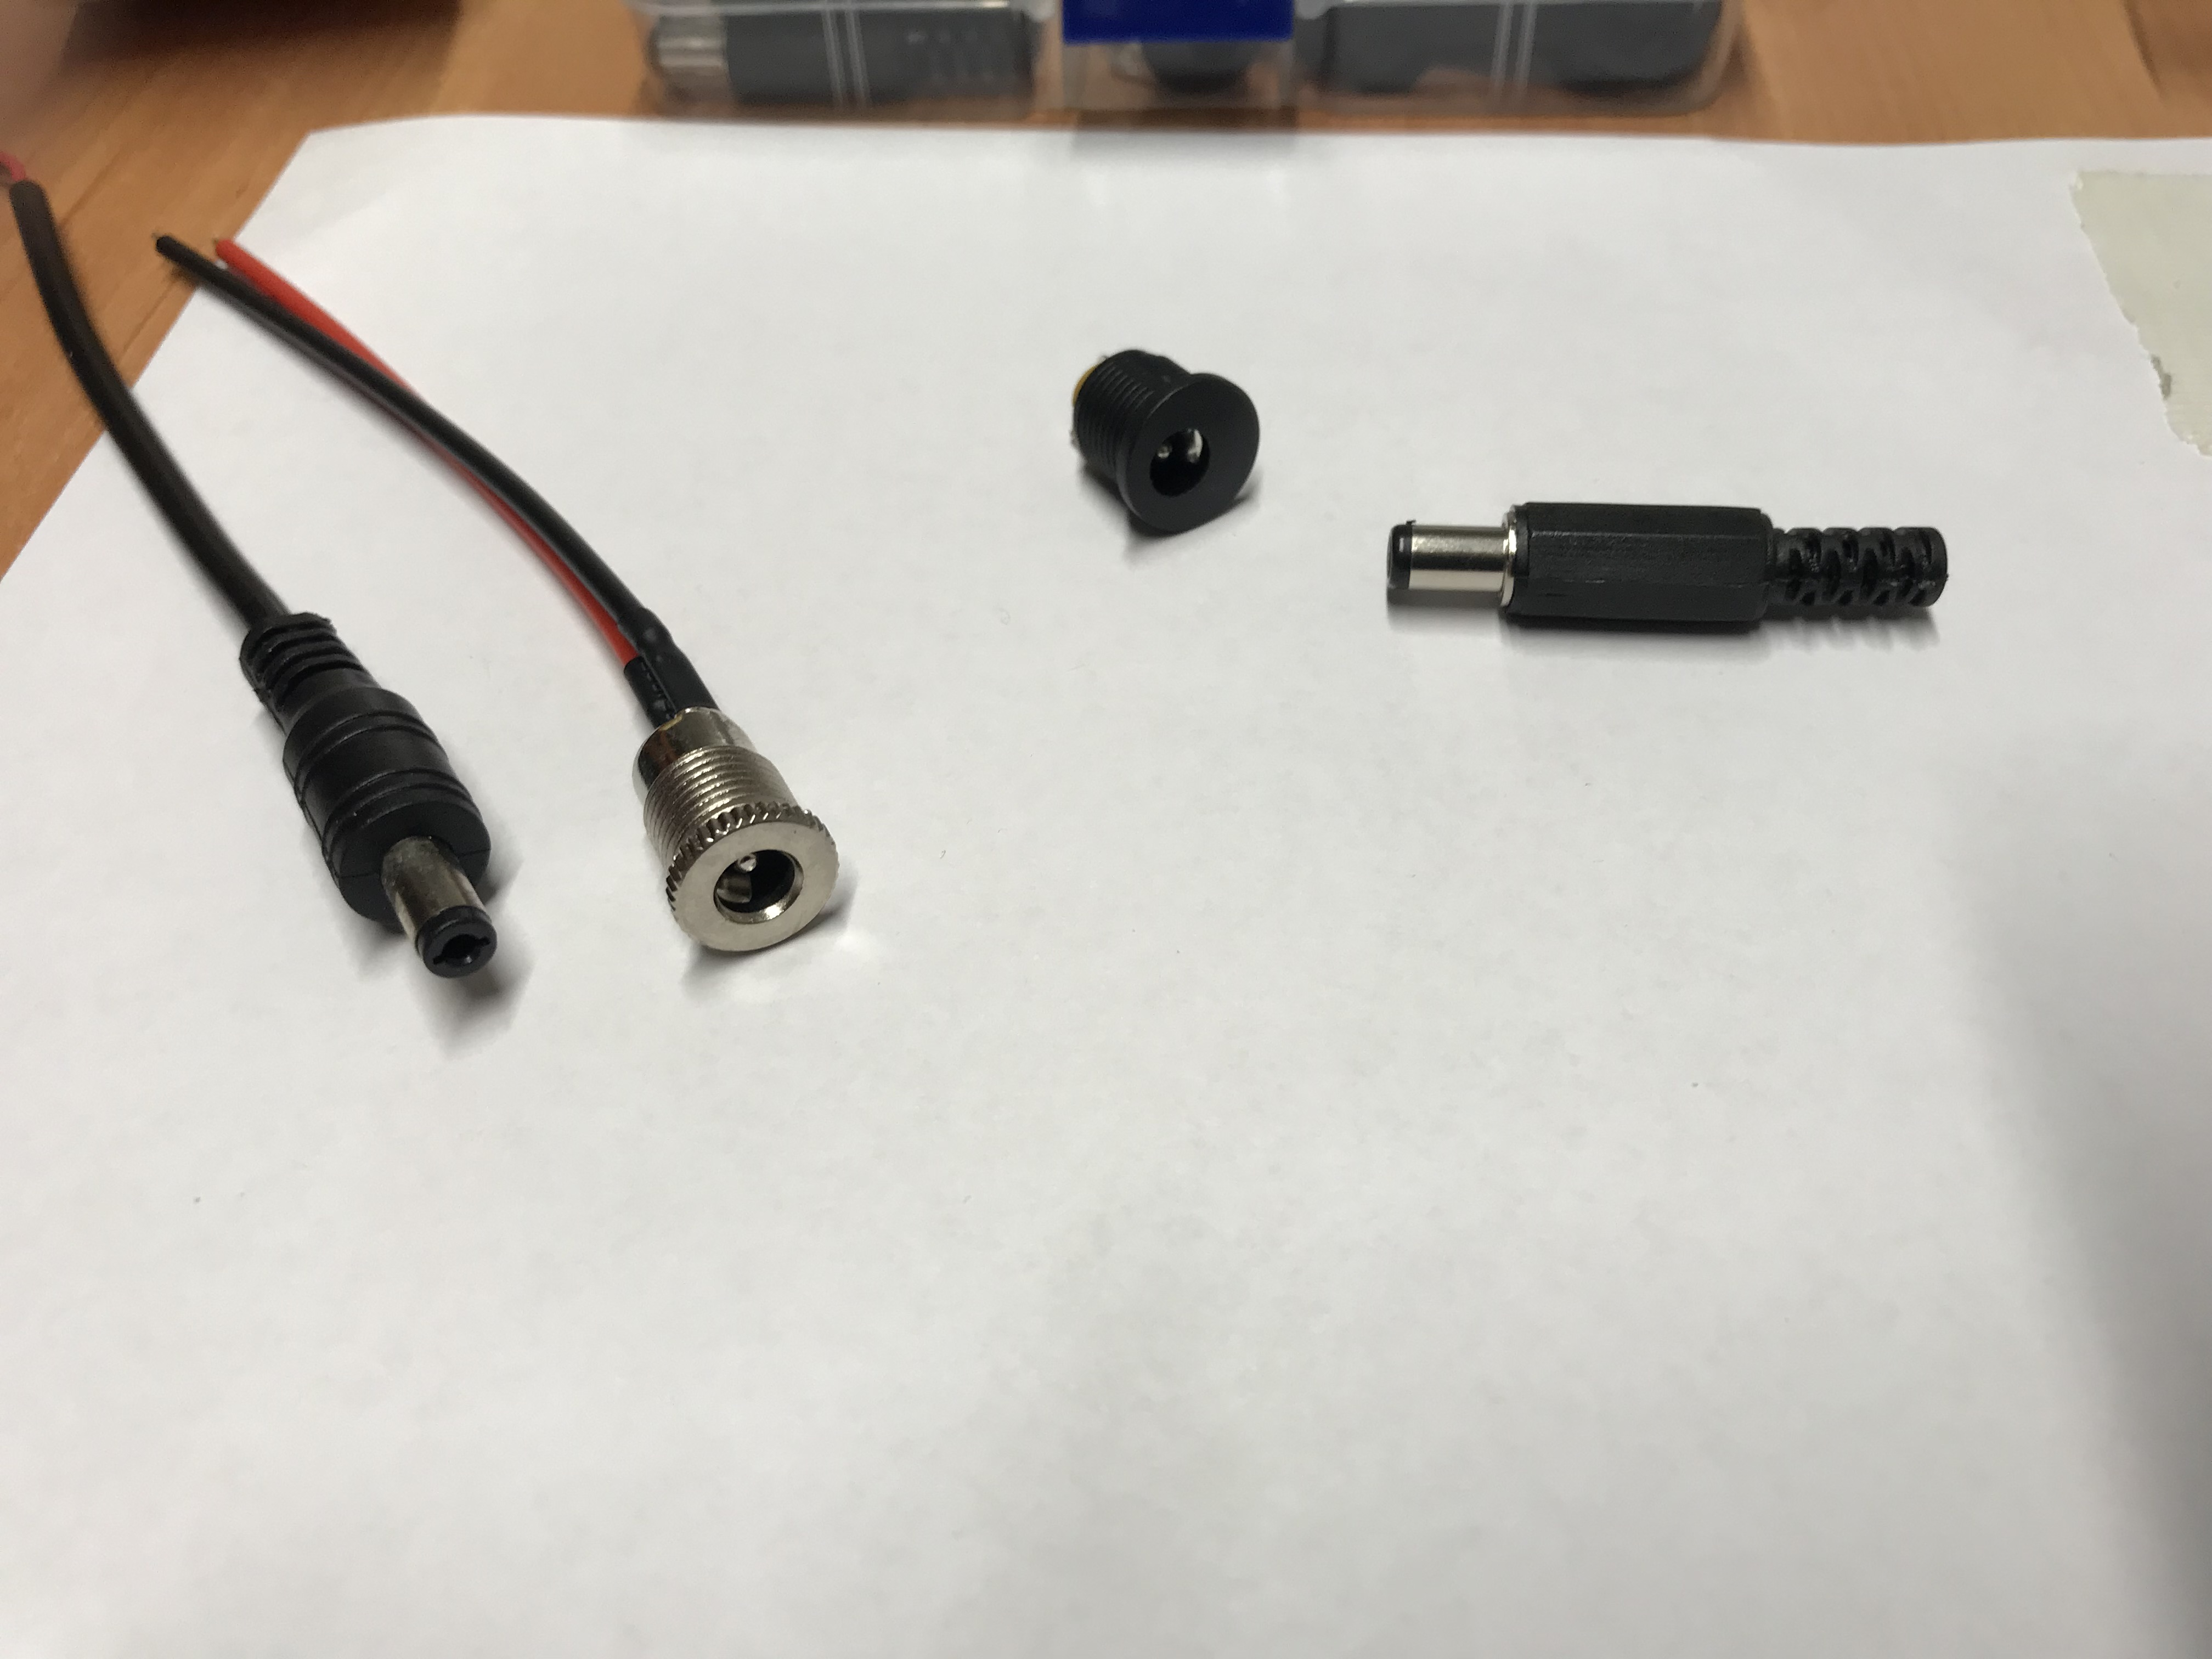
\includegraphics[scale=.05]{pictures/dcJack.jpg}};
            \end{scope}
        }{
            \draw (0,0) rectangle (3,1.5) ;
        }{Amazon}{Sin Id} {24V} {3A}
        \multirow{3}{*}{\makecell{Hembra \\ Socket}}
        \connectordata{
            \begin{scope}
                \clip (-1,-0.75) rectangle  +(2,1.5);
                \node[inner sep=0pt] at (-0.2,-1.7)
                    {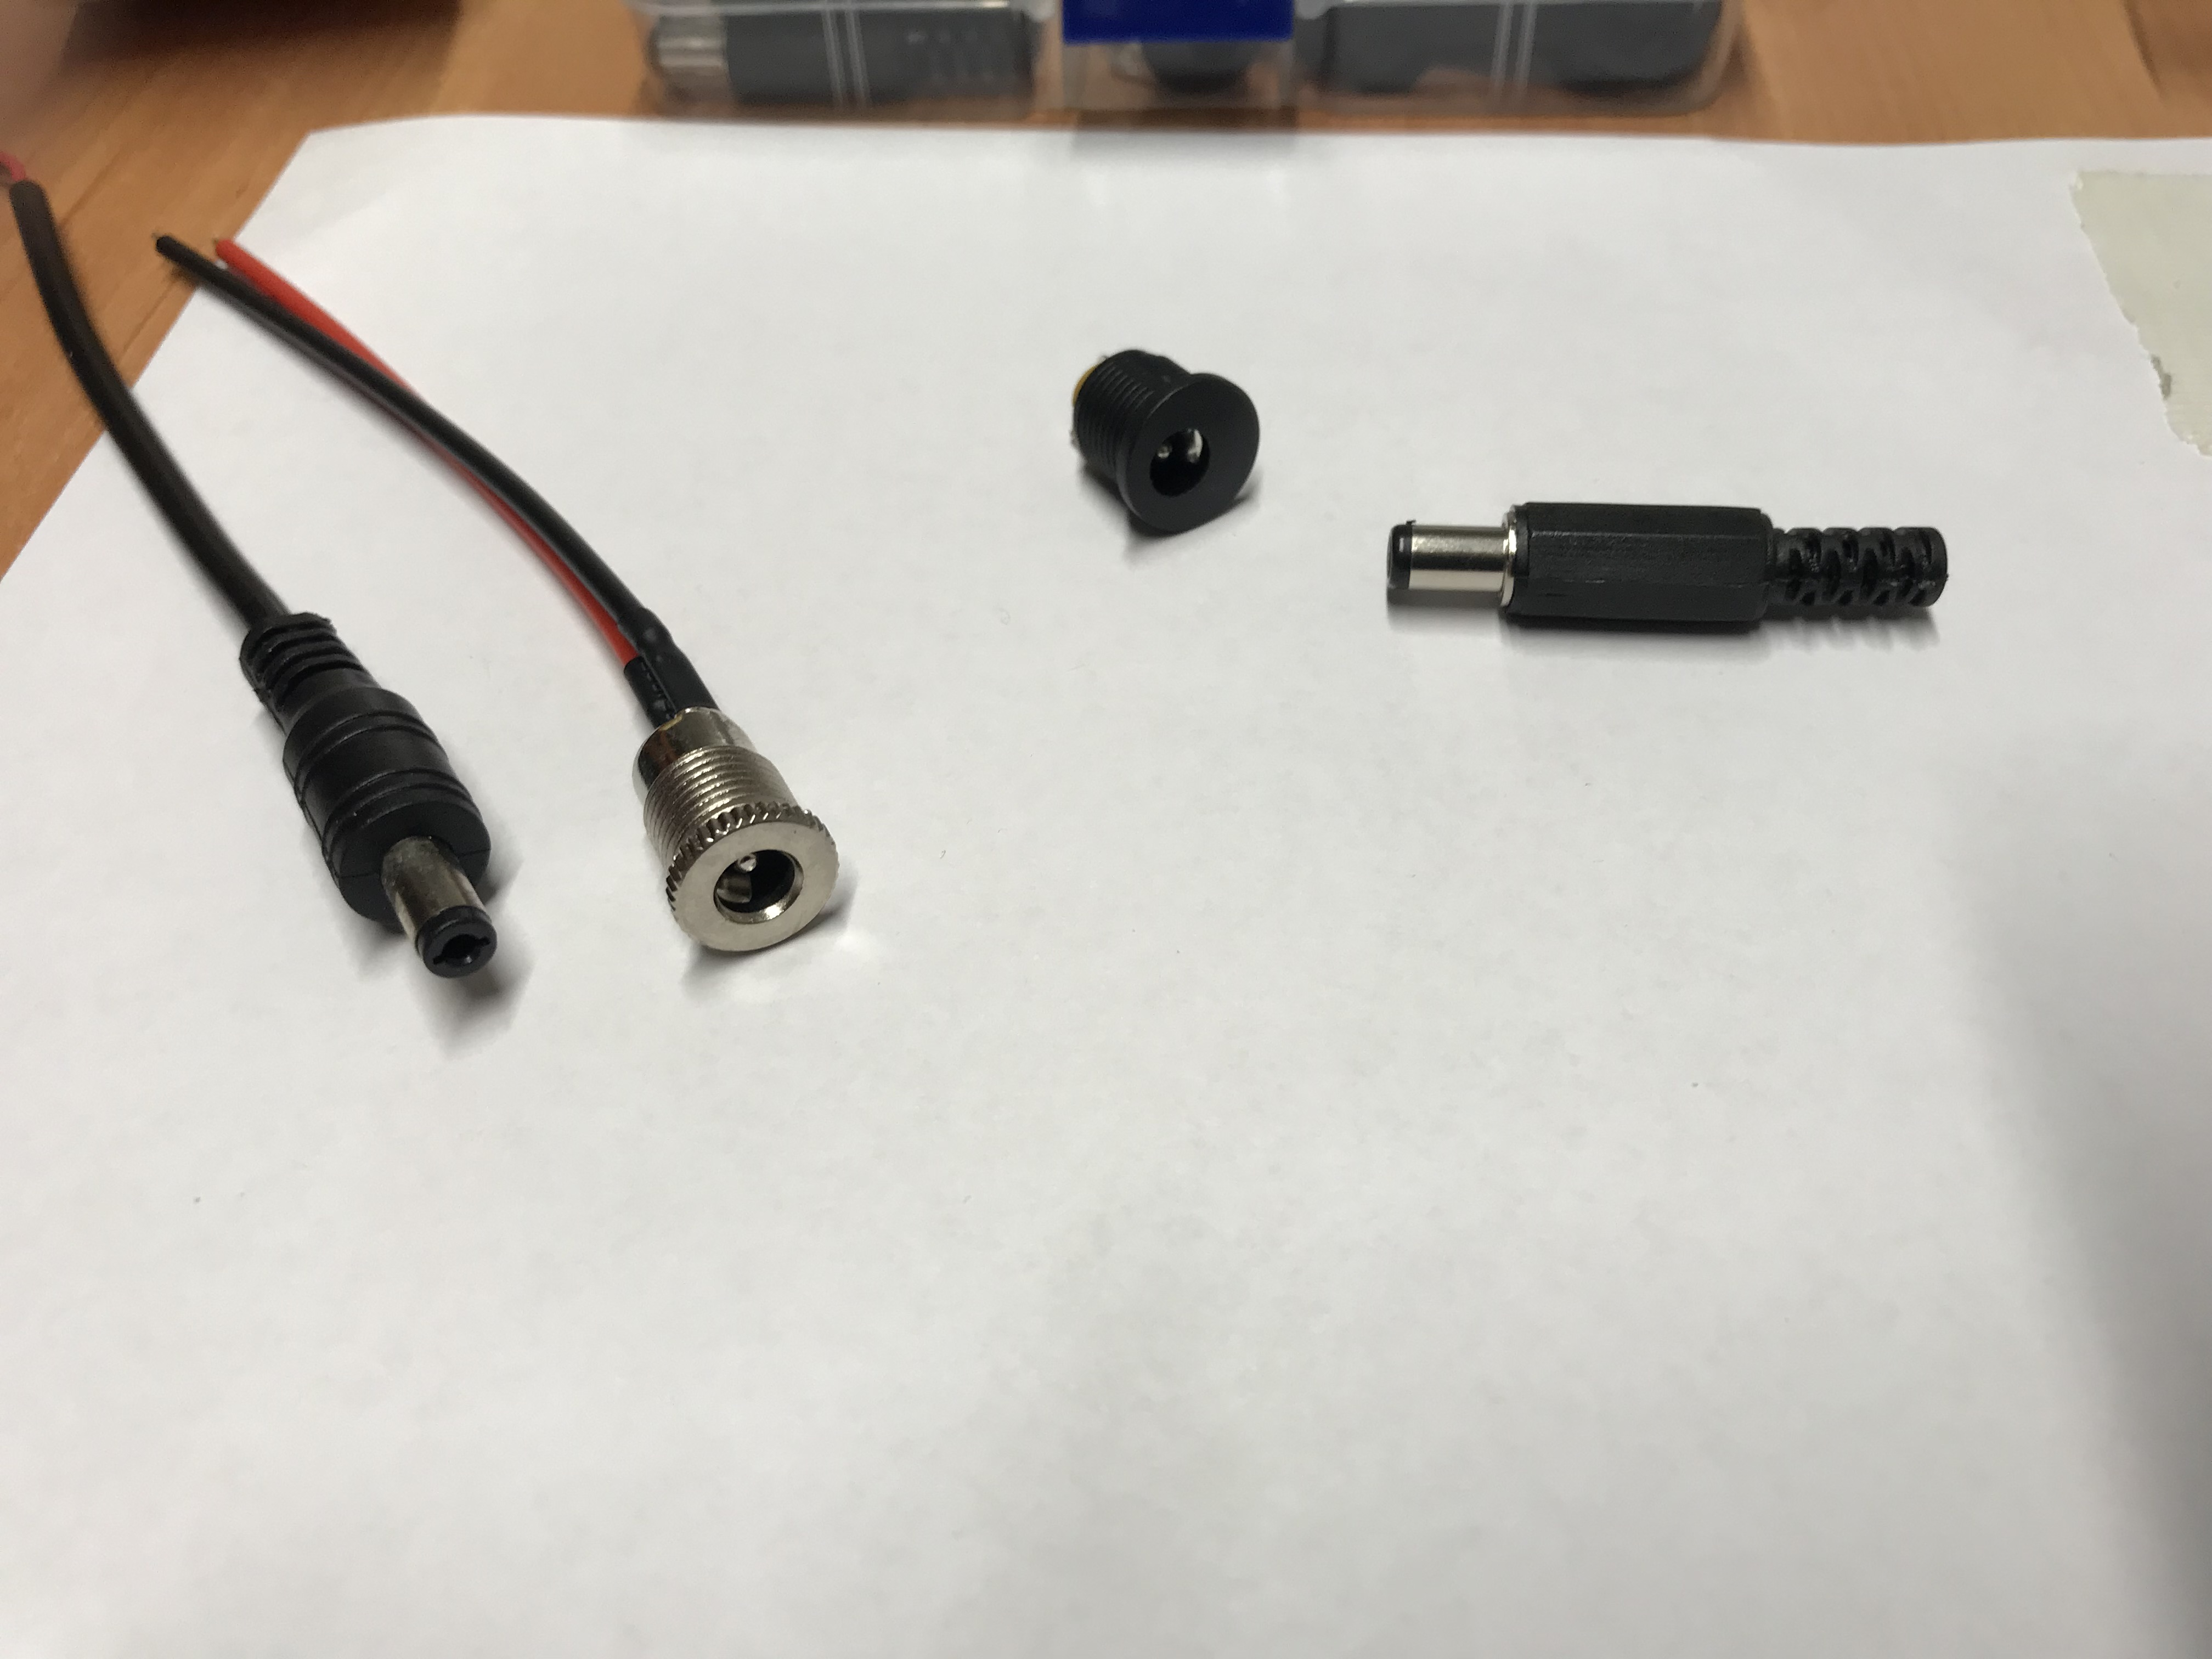
\includegraphics[scale=.07]{pictures/dcJack.jpg}};
            \end{scope}
        }{
            \draw (0,0) rectangle (3,1.5) ;
        }{Amazon}{Sin Id} {24V} {3A}

        \multicolumn{5}{|l|}{\makecell[l]{
            \tabitem Incluye tuerca para sujetar a panel \\
            \tabitem Incluye protector de goma
        }} \\
        \hline
    \end{tabular}
    \caption{Jack 2mm Amazon}
    \label{tab:DcJack1}
\end{table}

\begin{table}[H]
    \centering
    \renewcommand\theadfont{\bfseries}
    \setlength{\tabcolsep}{10pt}
    \renewcommand{\arraystretch}{1.5}

    \begin{tabular}{|c|c|c|c|c|}
        \beginConnectorTable{DC Jack 2mm}
        \multirow{3}{*}{\makecell{Macho \\ Plug}}
    
        \connectordata{
            \begin{scope}
                \clip (-1,-0.65) rectangle  +(2,1.3);
                \node[inner sep=0pt, rotate=60] at (1.3,2)
                    {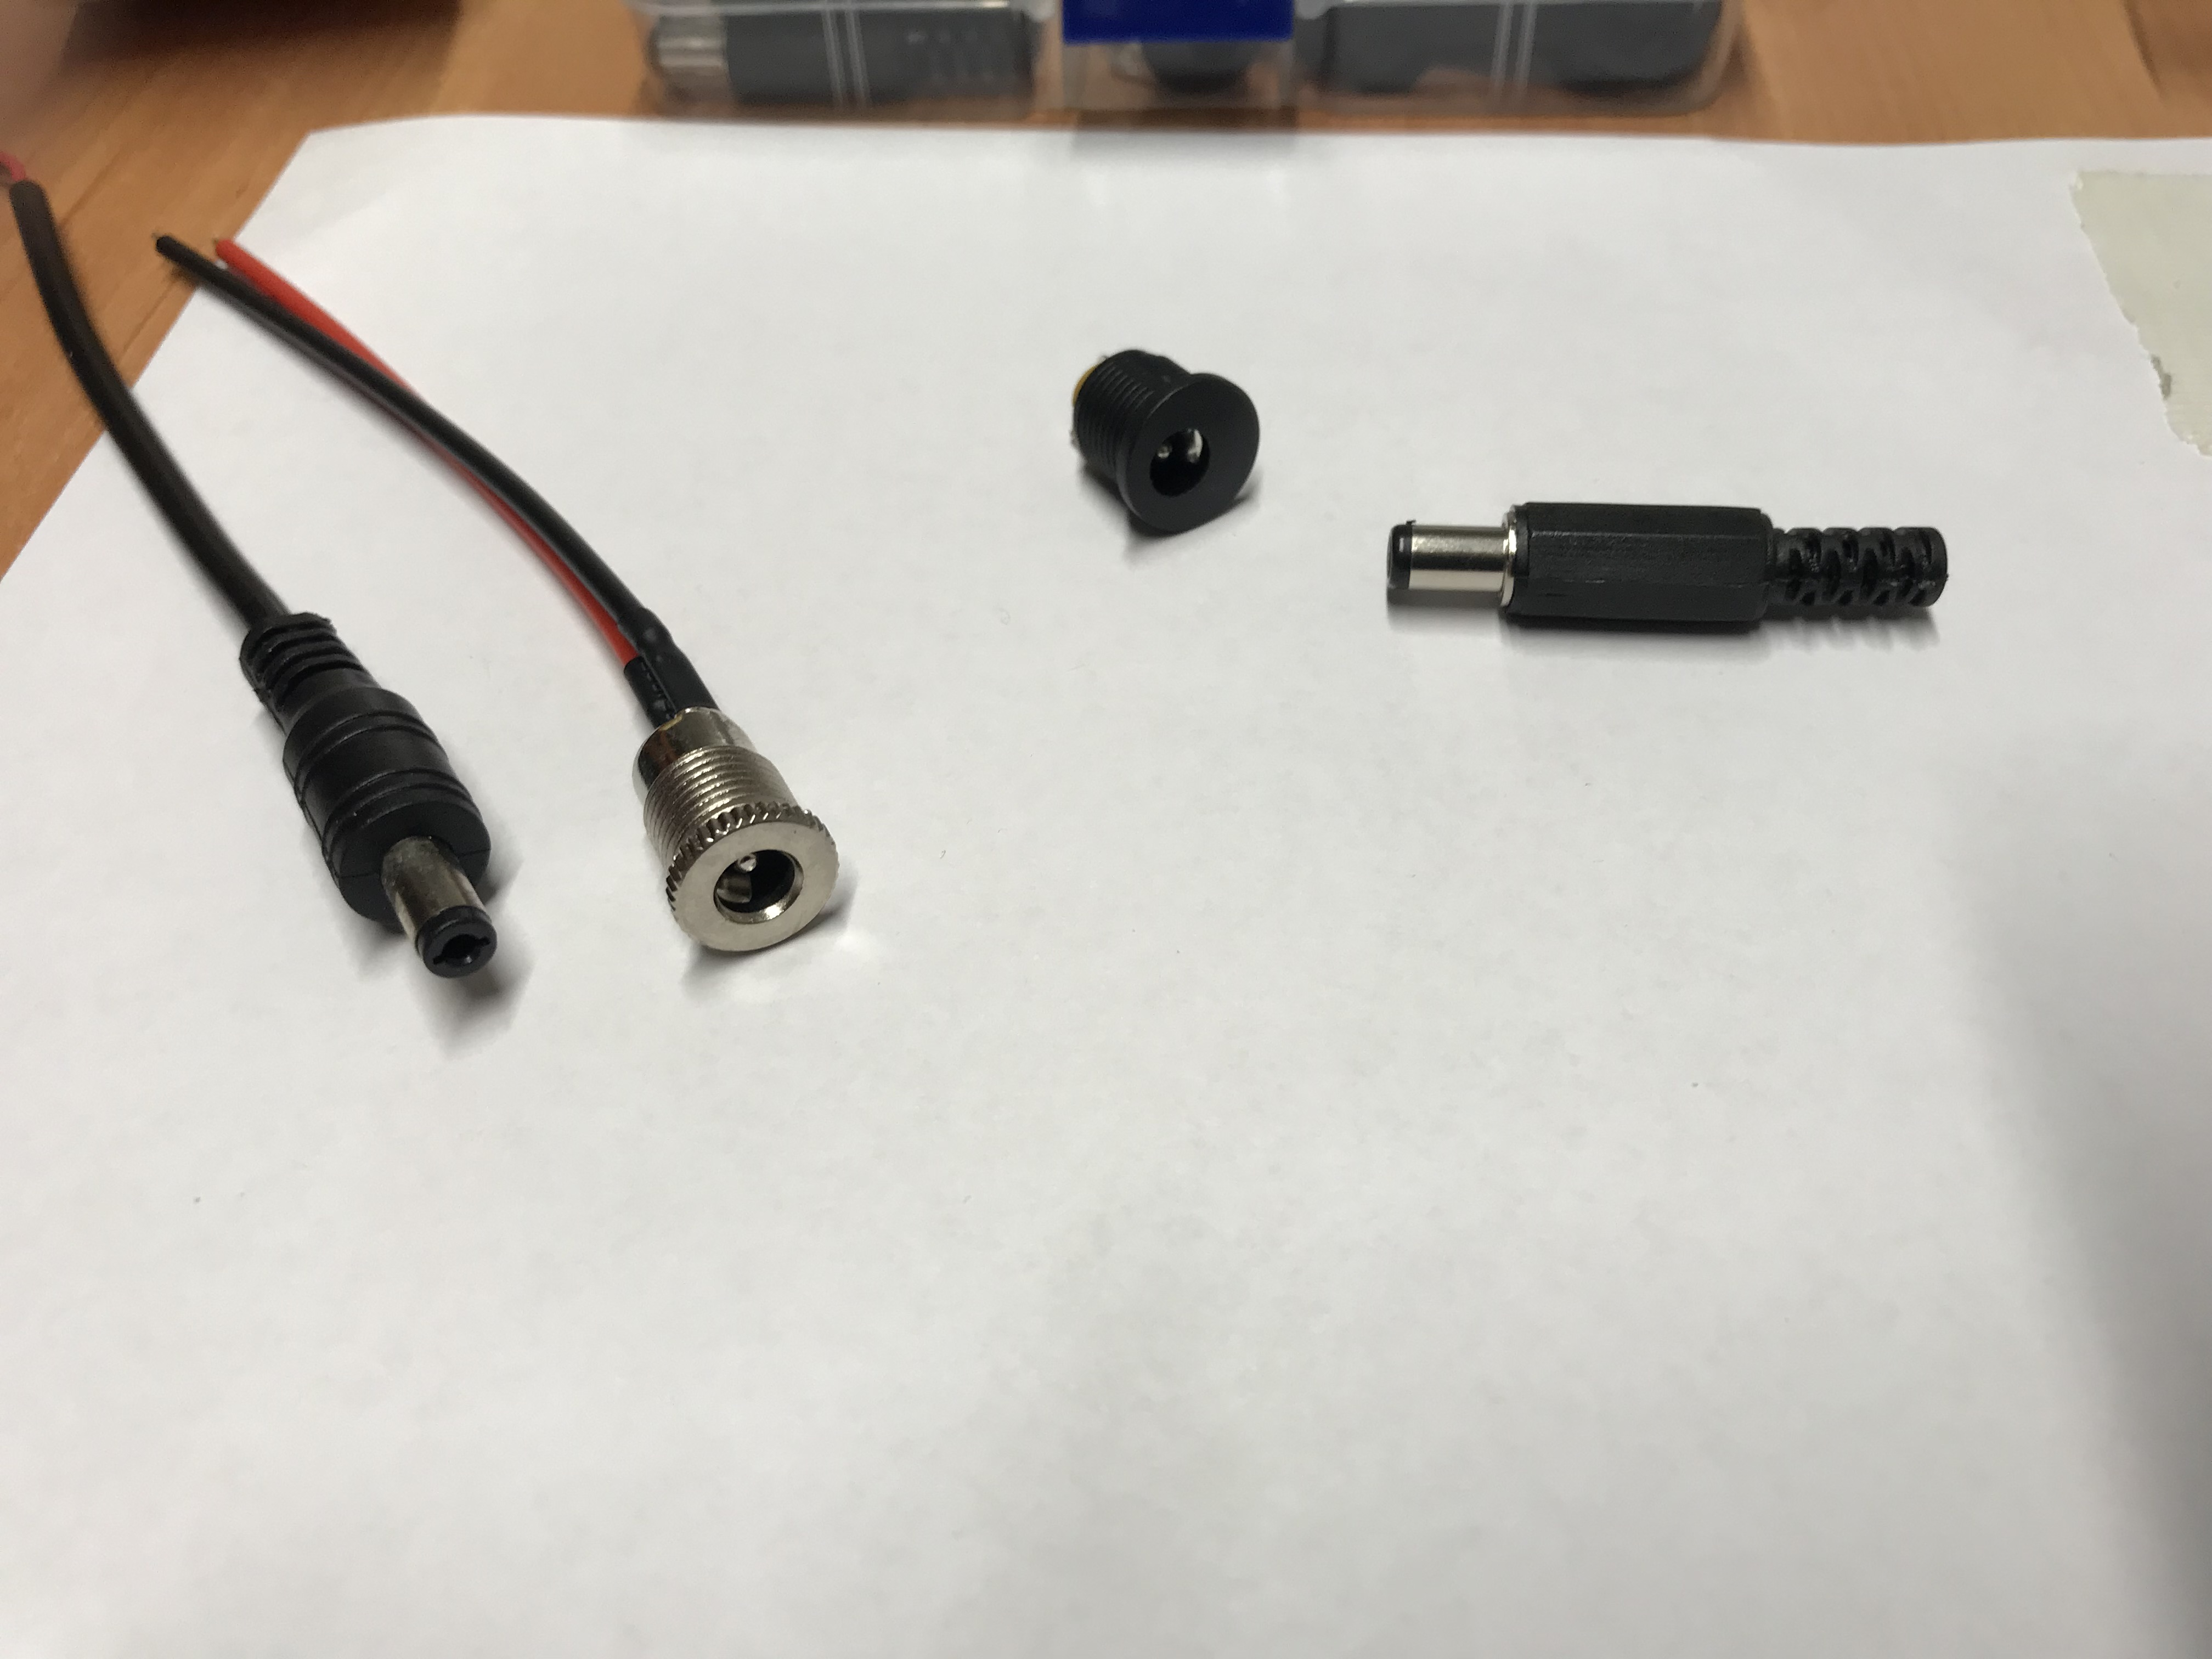
\includegraphics[scale=.05]{pictures/dcJack.jpg}};
            \end{scope}
           
        }{
            \draw (0,0) rectangle (3,1.5) ;
        }{Amazon}{Sin Id} {24V} {3A}
        \multirow{3}{*}{\makecell{Hembra \\ Socket}}
        \connectordata{
            \begin{scope}
                \clip (-1,-0.65) rectangle  +(2,1.3);
                \node[inner sep=0pt, rotate=60] at (0.9,1)
                    {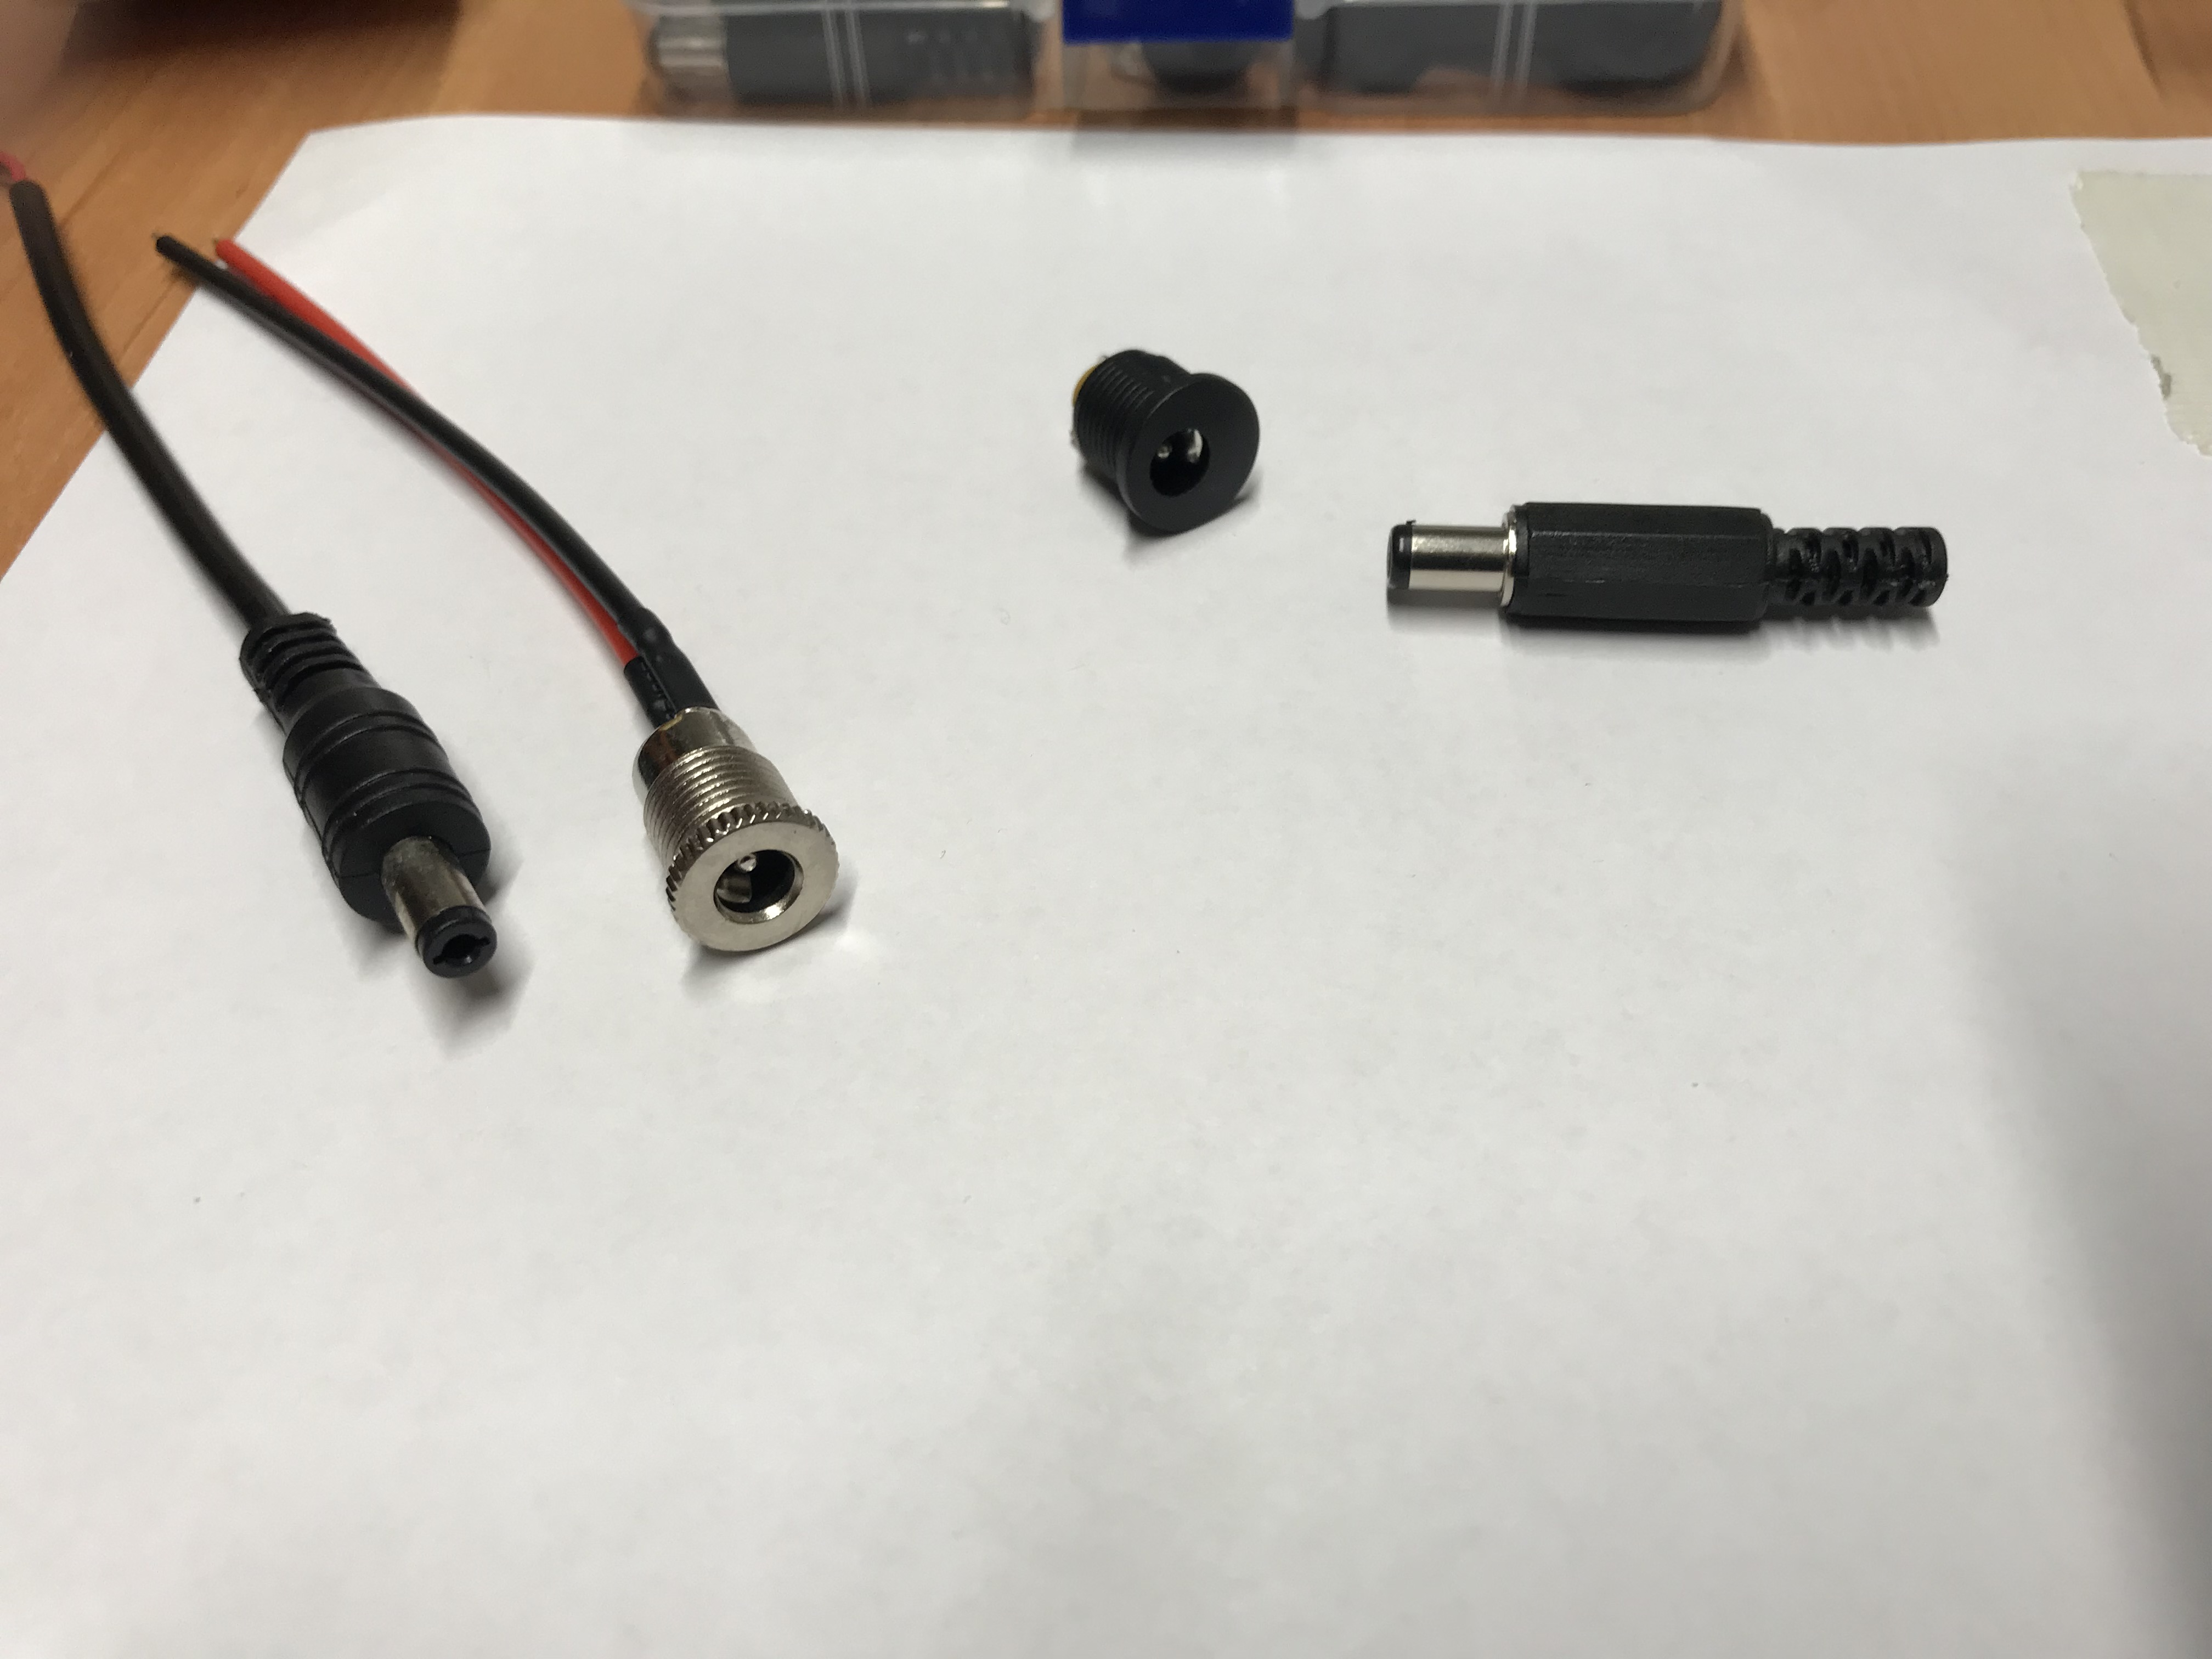
\includegraphics[scale=.05]{pictures/dcJack.jpg}};
            \end{scope}
        }{
            \draw (0,0) rectangle (3,1.5) ;
        }{Amazon}{Sin Id} {24V} {3A}

        \multicolumn{5}{|l|}{\makecell[l]{
            \tabitem Incluye tuerca para sujetar a panel \\
            \tabitem Es de metal conectado a (-) \\
            \tabitem Cables pre-soldados
        }} \\
        \hline
    \end{tabular}
    \caption{Jack 2mm Amazon}
    \label{tab:DcJack2}
\end{table}


\begin{table}[H]
    \centering
    \renewcommand\theadfont{\bfseries}
    \setlength{\tabcolsep}{10pt}
    \renewcommand{\arraystretch}{1.5}


    \begin{tabular}{c |c |c |c |c |}
        entrada & \thead[b]{item} & \thead[b]{Recomendado} & \thead[b]{Maximo} & \thead[b]{Con Bypass} \\ 
        \Xhline{5\arrayrulewidth}
%Entrada DCC
        \rowcolor{Melon!15}
        & Voltaje &14-20V & \multicolumn{2}{c|}{12-24V} \\
        \cline{2 - 5}
        \rowcolor{Melon!10} \cellcolor{Melon!15}
        \multirow{-2}{*}{DCC}&Corriente & 1A & 1.5A & 2A \\ \Xhline{3\arrayrulewidth}
%Entrada Jack
        \rowcolor{blue!15} & Voltaje & 12-20V & \multicolumn{2}{c|}{10-24V} \\
        \cline{2 - 5}
        \rowcolor{blue!10} \cellcolor{blue!15} \multirow{-2}{*}{ \makecell{ \cellcolor{blue!15} Jack\\ \cellcolor{blue!15} Terminal}} & Corriente & 1A & 1.5A & 3A \\
        \Xhline{5\arrayrulewidth}
    \end{tabular}
    \caption{Limites de entrada}
    \label{tab:limiteEntrada}
\end{table}
\end{document}